\chapter{User interface design} \label{chap:userinterface}
As the product we are designing is intended to be distributed to general public, its user interfaces shall be friendly and appealing. Nevertheless, the purpose of this document is to guide the many professionals who will work on the project, without excessively constraining their abilities and creativity. For this reason, we are going to provide some mock-ups of the two mobile applications (myTaxiWeb is omitted, for the sake of compactness, as it does not offer to users anything more than myTaxiApp). The following mock-ups should be intended as a reference for the structure of each screen, and by no means shall be used as an ``artistic'' model.

While working on the user interfaces for this project, the requirements expressed in the RASD in paragraph~2.1.2 and in section~2.3 must be taken into consideration, together with this chapter.


\section{myTaxiApp}
Upon opening the application, the user is presented with the following options: log in the system, sign up, and request a taxi ride (as a guest).

\begin{figure}%
	\hfill%
	\fbox{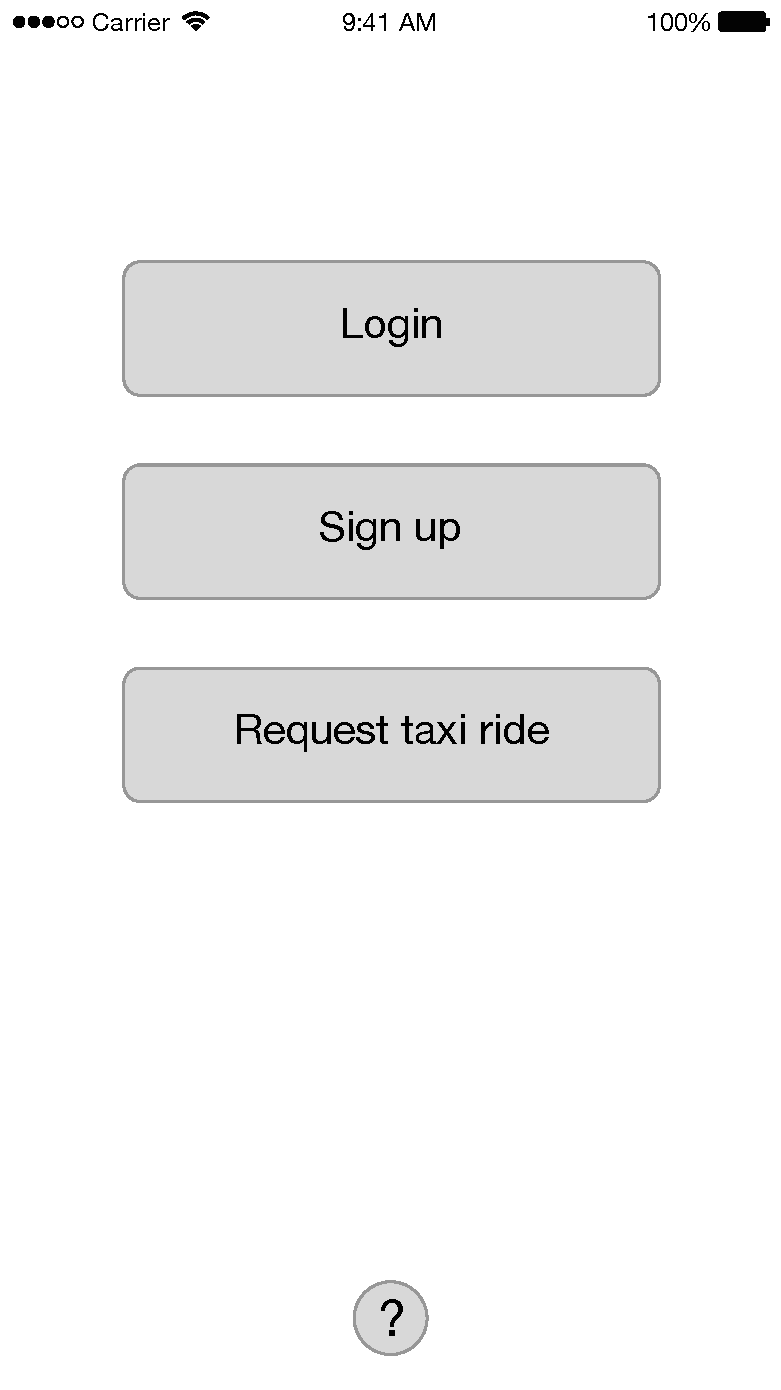
\includegraphics[page=1,width=\MuW\linewidth]{img/mTS_iOS}}%
	\hfill%
	\caption{Home page, presented to the user after his opening the application.}\label{fig:firstPage}
\end{figure}

\newpage 

If he chooses to log in, then he will need to fill in the form with his email and password details. Obviously he needs to be registered on the system, otherwise the login procedure will fail. Should he not be registered, he can sign up, by providing some personal details (name, phone number, email).

\begin{figure}%
	\hfill%
	\fbox{\includegraphics[page=2,width=\MuW\linewidth]{img/mTS_iOS}}%
	\hfill%
	\fbox{\includegraphics[page=4,width=\MuW\linewidth]{img/mTS_iOS}}%
	\hfill%
	\caption{Login and Sign up pages.}\label{fig:loginSignup}
\end{figure}

After the login, the user (now he is identified in the system as a registered customer) has the possibility to request or reserve a taxi, manage his favourite addresses (a convenient feature which lets users to save some addresses, for a faster retrieval).

\begin{figure}%
	\hfill%
	\fbox{\includegraphics[page=3,width=\MuW\linewidth]{img/mTS_iOS}}
	\hfill%
	\caption{Registered customer's home page.}\label{fig:logged}
\end{figure}

\newpage

Actually, the screen which allows to request a taxi is the same for registered and guest users, as origin, destination and number of people shall be specified in both cases. However, we have to make some distinctions: only registered customers can select favourite addresses as origin and destination; name and number details are requested only to guest users. 

\begin{figure}%
	\hfill%
	\fbox{\includegraphics[page=5,width=\MuW\linewidth]{img/mTS_iOS}}%
	\hfill%
	\fbox{\includegraphics[page=10,width=\MuW\linewidth]{img/mTS_iOS}}%
	\hfill%
	\caption{Request a taxi ride (mind the distinctions for registered and guest users).}\label{fig:request}
\end{figure}

Registered users are given the possibility to reserve a taxi ride. This means that they have to select date and time for the ride. 

\begin{figure}%
	\hfill%
	\fbox{\includegraphics[page=6,width=\MuW\linewidth]{img/mTS_iOS}}%
	\hfill%
	\caption{Reserve a taxi ride.}\label{fig:reservation}
\end{figure}

\newpage

Also, registered users can have a list of favourite addresses, which they can manage by adding, deleting and editing addresses.

\begin{figure}%
	\hfill%
	\fbox{\includegraphics[page=7,width=\MuW\linewidth]{img/mTS_iOS}}%
	\hfill%
	\fbox{\includegraphics[page=8,width=\MuW\linewidth]{img/mTS_iOS}}%
	\hfill%
	\caption{Manage the list of favourite addresses.}\label{fig:manageAddresses}
\end{figure}

Finally, registered users can obviously manage their own account by changing the phone number, email address or password, and even delete the account (these functions are not expanded since trivial).

\begin{figure}%
	\hfill%
	\fbox{\includegraphics[page=9,width=\MuW\linewidth]{img/mTS_iOS}}%
	\hfill%
	\caption{Manage account.}\label{fig:manageAccount}
\end{figure}

\newpage

\section{myTaxiAssist}

\lipsum[1-2]
